%
% einleitung.tex -- Beispiel-File für die Einleitung
%
% (c) 2020 Prof Dr Andreas Müller, Hochschule Rapperswil
%
\section{Einleitung\label{pade:section:einleitung}}
\rhead{Einleitung}
Für praktische Berechnungen von Modellen in der Physik, Ingenieurwissenschaften und weiteren Gebieten wird die Taylor-Reihe schon früh im Studium als ein nützliches Werkzeug gelehrt.
Leider liefert die Taylor-Reihe nicht immer eine genügend gute Approximation.
Dieses Paper beschäftigt sich mit der Padé-Approximation, welche aus gebrochen rationalen Funktionen besteht und oft in der Notation
\begin{equation*}
[L/M]
=
\frac{P_{L}(x)}{Q_{M}(x)},
\end{equation*}
angetroffen wird. 
Die Definition dieser Notation wird im Abschnitt \ref{pade:subsection:Pade_erstellen} erläutert.
Padé-Approximationen sind Brüche, welche nur wenig komplizierter als Taylor-Reihen sind und ergänzen somit die Taylor-Reihe als Approximationsmethode.
Die Padé-Approximation kann gewisse Funktionen besser approximieren als Polynome, denn Polynome gehen immer gegen $\infty$ während Brüche beschränkte Funktionen approximieren können.
Wenn die Taylor-Reihe keine genügenden Ergebnisse liefert, kann die Padé-Approximation verwendet werden, um die Approximation zu verbessern.

 

\subsection{Das Taylor-Reihen Problem
\label{pade:Taylorfehler}}

Eine konvergente Taylor-Reihe definiert den Wert einer Funktion, welche beliebig oft abgeleitet werden kann. 
In der Praxis wird die Funktion jedoch nur mit immer längeren Polynomen approximiert da wir keine unendlich lange Polynome verwenden können.
Diese Vorgehensweise kann bei praktischen Problemen auch einen sehr unerwünschten und limitierenden Effekt haben. 
Schauen wir das Beispiel 
\begin{equation*}
f(x)
=
\left(\frac{1+2x}{1+x}\right)^{\frac{1}{2}}
\approx
1+\frac{1}{2}x - \frac{5}{8}x^2+\frac{13}{16}x^3 -\frac{141}{128}x^4 +\frac{399}{256}x^5 - \frac{2353}{1024}x^6 + \frac{7205}{2048}x^7 \mp \cdots
\end{equation*}
an. 

Die originale Funktion $f(x)$ ist eine zwischen $0<x<\infty$ einfache und stetige Funktion, welche sich von $1$ zu $\sqrt{2}$ bewegt.
Die dazugehörige Taylor-Reihe konvergiert für $x>\frac{1}{2}$ nicht. 
Das Verhalten der originalen Funktion und deren Taylor-Reihe ist in dem Graphen \ref{pade:prob1} ersichtlich. 

\begin{figure}
	\centering
	\subfigure[Plot von $f(x)$ und Taylor-Reihe 7. Ordnung.\label{pade:prob1}]{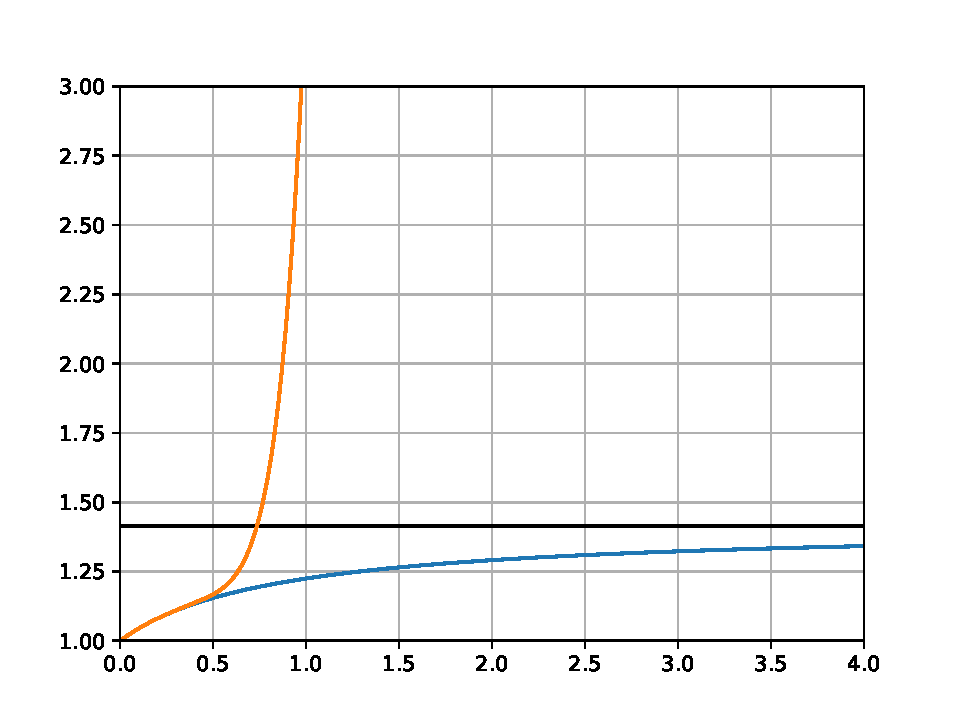
\includegraphics[width=0.45\linewidth]{./papers/pade/python/bilder/taylorProb1.pdf}}
	\subfigure[Fehler zwischen der Funktion und der Approximation.\label{pade:prob2}]{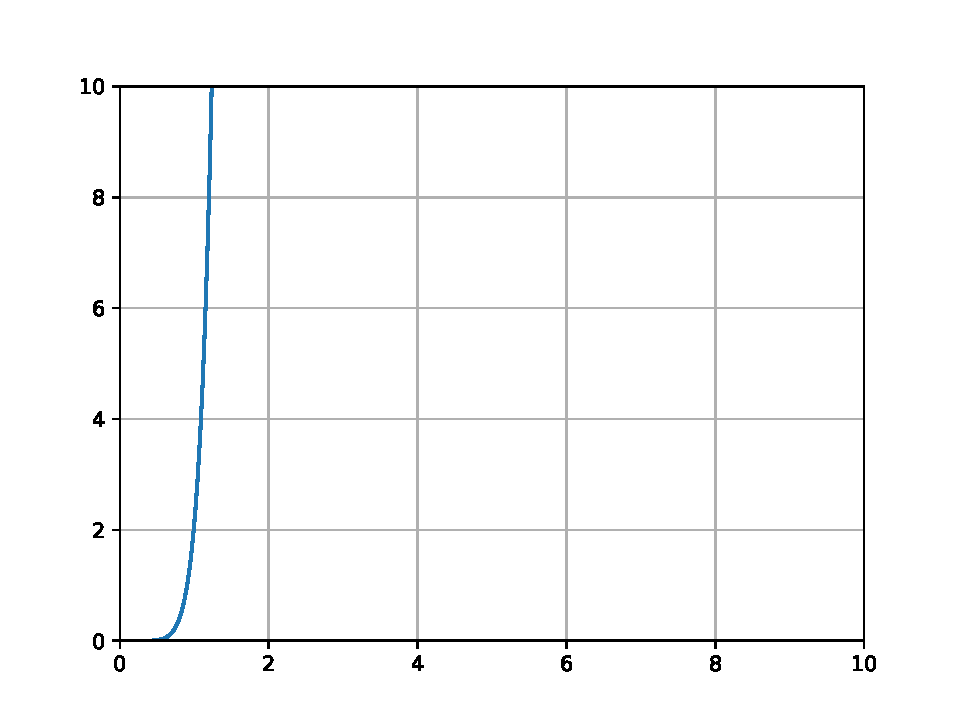
\includegraphics[width=0.45\linewidth]{./papers/pade/python/bilder/taylorProb3.pdf}}
	\subfigure[Plot von $f(x)$ und Padé-Approximation 3. Ordnung.\label{pade:prob3}]{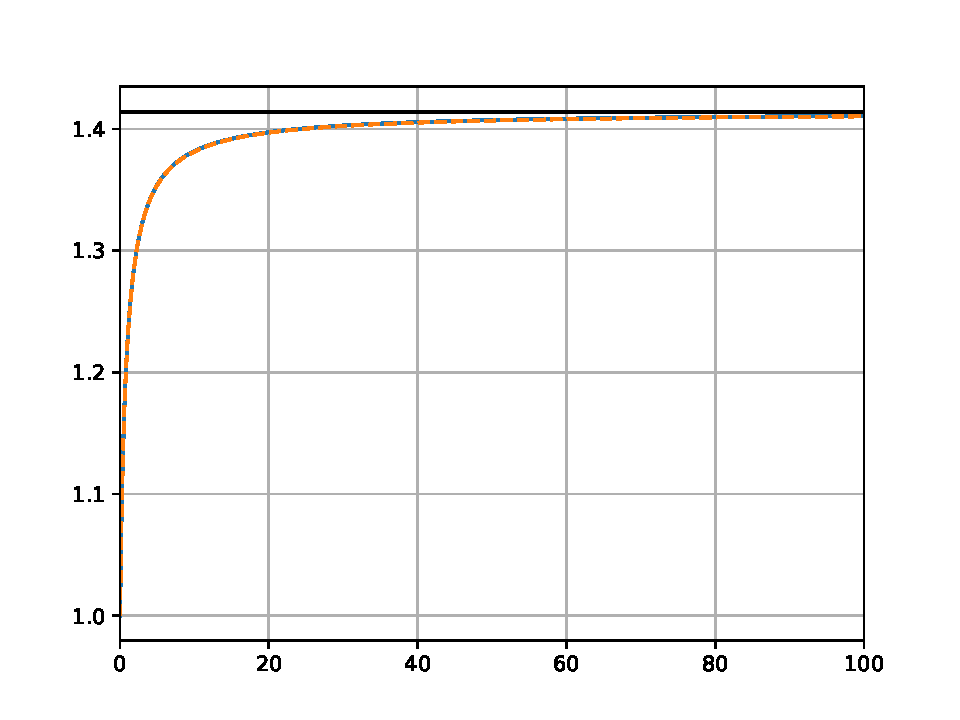
\includegraphics[width=0.45\linewidth]{./papers/pade/python/bilder/taylorProb2.pdf}}
	\subfigure[Fehler zwischen der Funktion und der  Padé-Approximation 3. Ordnung.\label{pade:prob4}]{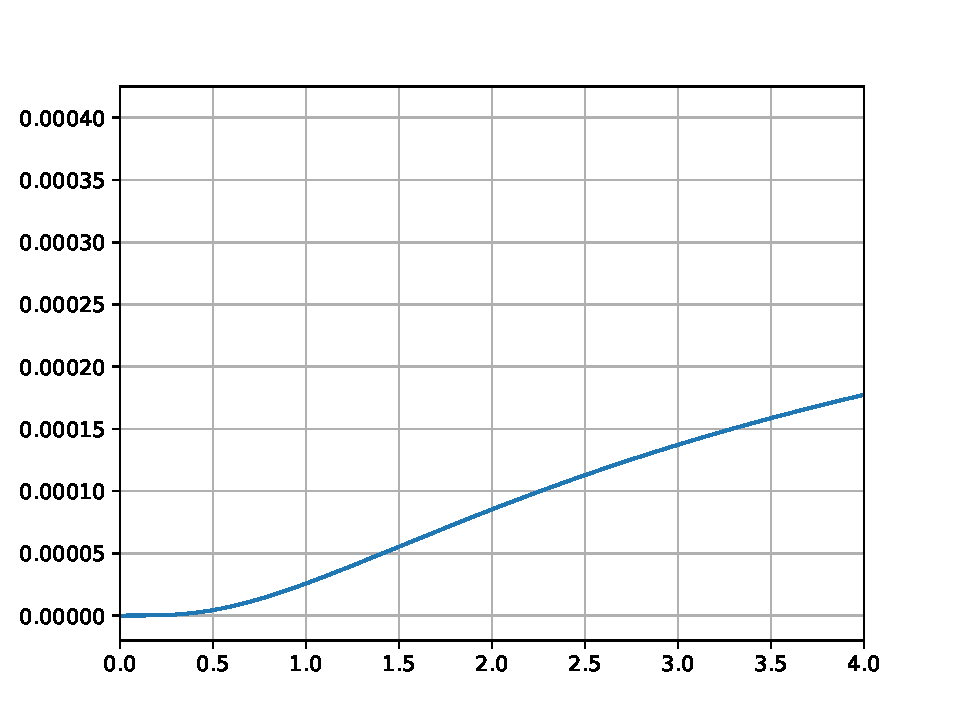
\includegraphics[width=0.45\linewidth]{./papers/pade/python/bilder/taylorProb4.pdf}}
	\caption{Visualisierung der Funktion $f(x)$ und ihren Approximationen \label{pade:prob}}
\end{figure}
Die Padé-Approximation ist eine spezielle Art von rationalen Brüchen, welche eine Funktion approximiert.
Diese Art der Approximation führt oft zu einem besseren Resultat als eine Taylor-Reihe. 
Manchmal können mit der Padé-Approximation auch dann gute Ergebnisse gewonnen werden, wenn eine Taylor-Reihe wie in diesem Beispiel nicht konvergiert. 

Wenn man aus den Koeffizienten der Taylor-Reihe nun eine Padé-Approximation erstellt 
\begin{equation*}
R_{[2/ 2]}(x)
=
\frac{P^{[2/2]}(x)}{Q^{[2/2]}(x)}
=
\frac{1+\frac{13}{4}x+\frac{41}{16}x^2}{1 + \frac{11}{4}x + \frac{29}{16}x^2} 
\label{pade:bspordnung2}
\end{equation*}
und diese Approximation bei immer grösser werdendem $x$ betrachtet
\begin{equation*}
\lim_{x \to \infty}
\left(
\frac{1+\frac{13}{4}x+\frac{41}{16}x^2}{1 + \frac{11}{4}x + \frac{29}{16}x^2} 
\right)
=
\frac{49}{29} = 1.413793103,
\end{equation*}
erhält man ein Ergebnis, welches sehr nahe an der originalen Funktion liegt. 
In der Grafik \ref{pade:prob3} ist gut ersichtlich, wie viel besser sich die Padé-Approximation im Vergleich zu der Taylor-Approximation verhält.
Wenn die beiden Fehler der Taylor-Reihe \ref{pade:prob2} und der Padé-Approximation \ref{pade:prob4} zur originalen Funktion betrachtet werden, kann man sehen, dass die Padé-Approximation deutlich besser ist.
Dies obwohl von der originalen Funktion nicht mehr Informationen bekannt waren als bei der Taylor-Reihe, da das Polynom ja aus der Taylor-Reihe erstellt wurde.

In den folgenden Abschnitten wird nun inklusive einiger Beispiele aufgezeigt, wie man eine Padé-Approximation erstellt.
Zum besseren Verständnis wird zuerst erklärt wie die Potenzreihe einer Funktion gefunden werden kann.










